\chapter{Related Work}\label{chap:relatedwork}
The fundamental ideas of gamification, its uses in educational contexts, and its prior research in the area of game-based learning are covered in this chapter. It also talks about the possible advantages and difficulties of gamification in the classroom, emphasizing the necessity for easily accessible resources that let teachers design customized gamified lessons. Gamification is the practice of integrating game-like elements into non-game settings to motivate and engage users. By incorporating features such as points, badges, leaderboards, challenges, and rewards, gamification transforms the user experience into an interactive and rewarding process that encourages participation and achievement. Gamification has been widely used in various domains, such as marketing, health, fitness, and education, to motivate users, drive behavior change, and enhance engagement. In education, gamification has gained popularity as a means of boosting student motivation, fostering engagement, and improving learning outcomes. Research has shown that gamification can enhance student performance, increase motivation, and reduce dropout rates across different educational levels and subjects \cite{lara2023badges}. For example, a study conducted by Lara-Cabrera et al. (2023) found that gamified techniques, such as awarding 3D-printed badges, can enhance academic performance and reduce dropout rates, especially in STEM programs at the higher education level \cite{lara2023badges}. Another study published in the Journal of Educational Technology (2022) demonstrated that gamification can increase student engagement and motivation in flipped classrooms by promoting active learning and collaboration \cite{jack2024gamification}. These studies highlight the potential of gamification to transform the learning experience and create personalized and engaging learning activities that motivate students to take an active role in their education.

Game-based learning (GBL) is an educational approach that uses games to teach students about specific subjects, concepts, or skills. GBL combines educational content with game mechanics to create interactive and engaging learning experiences that motivate students to learn and retain information effectively. By incorporating elements such as challenges, rewards, competition, and feedback, GBL can enhance student engagement, motivation, and learning outcomes. GBL can be used in various educational settings, such as schools, universities, and training programs, to facilitate skill development, reinforce concepts, and promote active learning. For example, a literature review conducted by Fernando et al. (2024) found that GBL can enhance student motivation through immediate feedback, clear objectives, and a sense of achievement \cite{fernando2024}. These studies highlight the potential of GBL to transform the learning experience and create meaningful and enjoyable learning activities that extend beyond traditional teaching methods.

Gamification can be categorized into three primary types: content-based gamification, structural gamification, and game-based learning (GBL). Content-based gamification involves embedding game-like elements into existing educational content, such as quizzes, assignments, or lectures, to make learning more interactive and engaging. In contrast, structural gamification focuses on redesigning the overall learning environment by incorporating game-like mechanics, such as progress tracking, rewards, or challenges, to enhance student motivation and engagement \cite{fernando2024}.

Game-based learning (GBL) has been proven as an effecetive means of education and is equally as effecetive as traditional learning methods, as Gordillo et al. (2020) have shown \cite{sgame2020}. Another reaserch introduced a 3D game authoring tool for users with little to no programming knowledge using OpenAi's GPT-4, however the toolkit has not been tested by instructors or students \cite{horn2023}. The use of structural gamification was also used to make visualization of data more engaging and interactive, as shown by the work of Karuna et al. (2022), as The study explores using gamification elements to enhance user engagement in data collection, focusing on game design and behavioral data visualization, the study later  concluded that using gamification in data collection, especially through visual and interactive methods, can significantly enhance user engagement and data quality. \cite{karuna2019}. these studies, however, have not focused on the generation of games and were not tested on instructors.

As outlined by Fernando and Premadasa (2024), these approaches are central to understanding how gamification and GBL can be effectively employed in educating Generation Alpha. Their systematic literature review highlights how these methods influence learning outcomes by promoting active participation and fostering deeper engagement in educational settings \cite{fernando2024}. The procedural generation of challenges and content in GBL has also been explored by Khoshkangini et al. (2021), who developed an automated system that generates personalized challenges based on player preferences, progress, and performance. This system addresses existing limitations in gamified learning environments by providing tailored experiences that cater to individual needs and learning styles \cite{khoshkangini2021}. Another personalized gamification system was proposed by Noor et al. (2010), which explores the automatic generation of personalized levels for platform games, which uses procedural content generation to create unique game levels based on player preferences and performance \cite{noor2010}. None of these systems, however, provide educators with the tools to design their own gamified learning experiences, limiting their potential impact on classroom instruction.

A number studies have underlined the effectiveness of gamification in educational fields. For instance, the work by Lara-Cabrera et al. (2023) has shown that gamified techniques developed with 3D-printed badges had positive influences on performance but also reduced the rate of STEM programs dropouts \cite{lara2023badges}. Jack et al. (2024) assessed the efficiency of using gamification within flipped classroom learning environments and reported significant increases in students' engagement and motivation based on active learning efforts \cite{jack2024gamification}. Gameification and game-based learning follow game design approaches and frameworks to create a more engaging and interactive learning experience. Fernando et al. 2024 have accentuated the role of GBL for fostering student motivation through immediate feedback, clear objectives, and a sense of accomplishment. Thus, these findings have come to demonstrate the ever-changing potential of gamification in education; they provide proof that gamification can create meaningful and engaging learning experiences beyond those possible through conventional pedagogies as proposed by Kalmpourtzis et al. 2018 \cite{Kalmpourtzis2018}.

The Elemental Tetrad model by Schell (2008) expresses a perspective where the core elements of game design are composed of four parts: mechanics, aesthetics, story, and technology, which is shown in figure \ref{fig:elemental_tetrad} . This model provides a holistic view of game design processes and helps designers create engaging and immersive game experiences. In a game, the mechanics are the rules, set goals, and interactions that define how players will engage in the game. Aesthetics refers to the audiovisual elements that define the look and feel of the game. Story is the narrative or plot, if any, providing context for the player's motives. Technology refers to hardware and software used in the creation and running of the game. By considering these four elements in the game design process, designers are able to create engaging, immersive, and enjoyable games for players \cite{schell2008art}. The Elemental Pentad later proposed by Kalmpourtzis et al. 2018 is a framework that builds on the framework of Schell and adds the element of pedagogy as shown in figure \ref{fig:elemental_Pentad}, which is the science of teaching. This model provides a comprehensive view of the game design process and helps designers create engaging and immersive game experiences that are also educational. By considering these five elements in the game design process, designers can create games that are engaging, immersive, and educational for players \cite{Kalmpourtzis2018}.

\begin{figure}
    \centering
    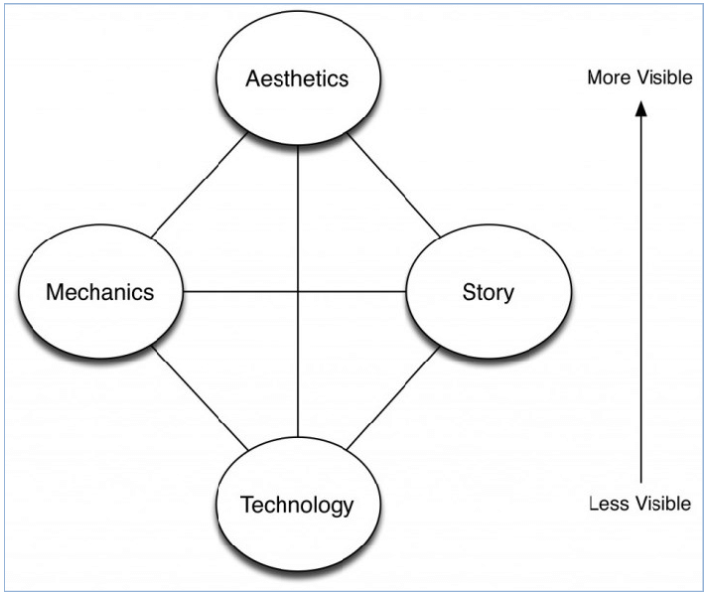
\includegraphics[width=0.8\textwidth]{figures/Related_Work/elem_tet.png}
    \caption{The Elemental Tetrad model by Schell (2008) \cite{schell2008art}}
    \label{fig:elemental_tetrad}
\end{figure}

\begin{figure}
    \centering
    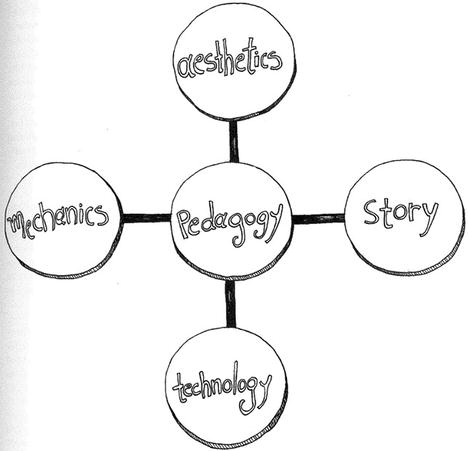
\includegraphics[width=0.8\textwidth]{figures/Related_Work/elem_pen.png}
    \caption{The Elemental Pentad model by Kalmpourtzis et al. 2018 \cite{Kalmpourtzis2018}}
    \label{fig:elemental_Pentad}
\end{figure}



Personalized gamification has also emerged as an exciting area of study, in which a procedurally generated system can create tailored goals and challenges for players based on their performance. The instructors have been also a great focus of gamification studies, as they could control what is being offered to the students, however, the tools available for them are still limited. For instance, The study by Gordillo et al. (2020) introduced a game-based learning platform that allows educators to create and share educational games with their students. The platform features a library of pre-built games and educational content covering various subjects and grade levels, making it easy for teachers to implement engaging learning activities in their classrooms \cite{sgame2020}.

Reza et al. presented an automated system that automatically generated customized challenges in accordance with the preference, progress, and performance of the learners to overcome some limitations found in already developed gamified systems \cite{khoshkangini2021}. Setting off these remarkable benefits, on the other hand, gamification is still an evolving area of study that boasts a number of challenges yet to be overcome. Probably one important limitation is that easy-to-use tools for educators who want to create gamified learning experiences without technical training in programming or game design are still in their infancy. Most of these systems are based on expert knowledge, making it hard for instructors who can't afford the resources or expertise necessary to implement gamified strategies themselves. User-centered tools in this respect could realistically let more educators take advantage of gamification, with further potentials to address a wide range from personalized and active learning settings.

In \emph{The Art of Computer Game Design}, Chris Crawford describes a game as an interactive medium where players make choices and experience the consequences of those choices. This definition is intentionally broad, encompassing various forms of games, such as board games, card games, sports, video games, and even educational games. Educational games, in particular, are designed to teach players about specific subjects, reinforce concepts, facilitate skill development, or help them understand historical events or cultures through gameplay \cite{crawford1982art}.

One of the closest works related to the work presented is the study by Gordillo et al. (2020) \cite{sgame2020}, which introduces a game-based learning platform designed for educators to create and share educational games with their students. The platform features a user-friendly interface that allows educators to create their own gamified education experience by combining two elements, the game and the educational contnet as shown in figure \ref{fig:sgame2020_creation}. Additionally, it includes a library of pre-built games covering various subjects and grade levels, making it easy for teachers to implement engaging learning activities in their classrooms. However, while Gordillo et al.’s work primarily focuses on game-based learning with preset game templates and pre-defined educational content, that does not allow for the creation of games with custom educational content. The gameplay also lacks the ability to integrate the educational content into it, rather the educational content is presented as a question after each level of the game shown in figure \ref{fig:sgame2020_gameplay}. This limitation restricts the platform’s potential for creating personalized learning experiences tailored to individual student needs and learning styles.

\begin{figure}
    \centering
    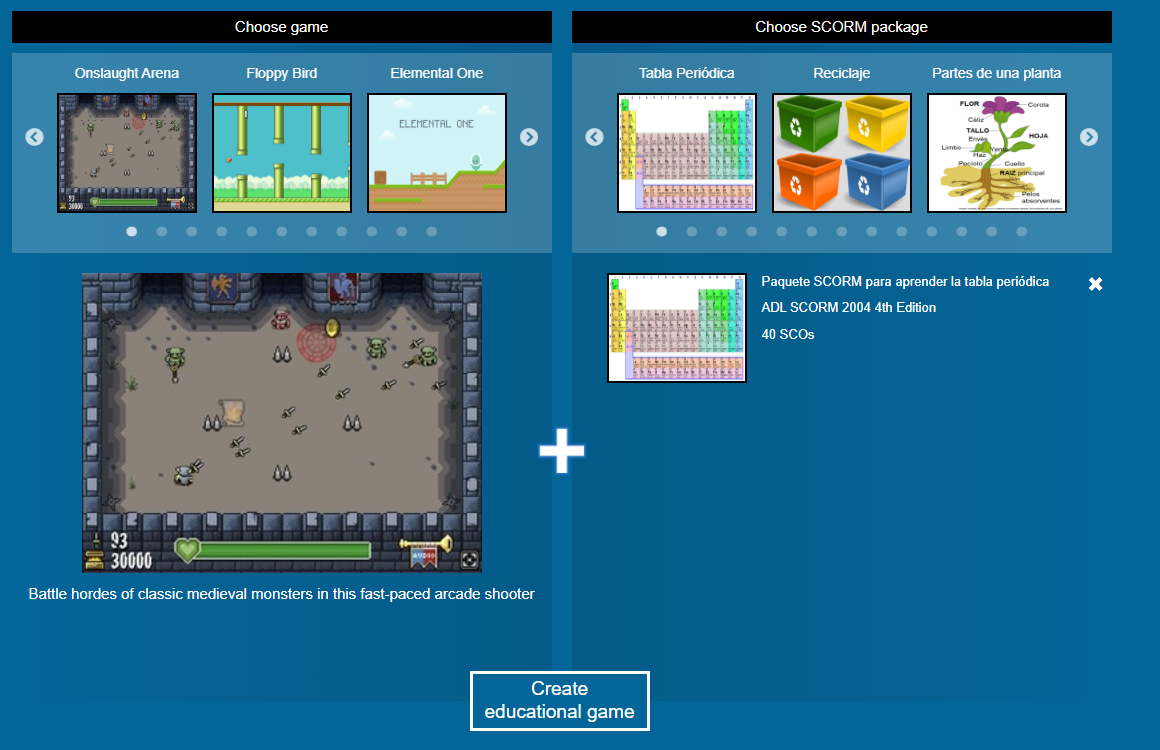
\includegraphics[width=0.8\textwidth]{figures/Related_Work/Sgame_creation.png}
    \caption{Educational game creation platform by Gordillo et al. (2020) \cite{sgame2020}}
    \label{fig:sgame2020_creation}
\end{figure}

\begin{figure}
    \centering
    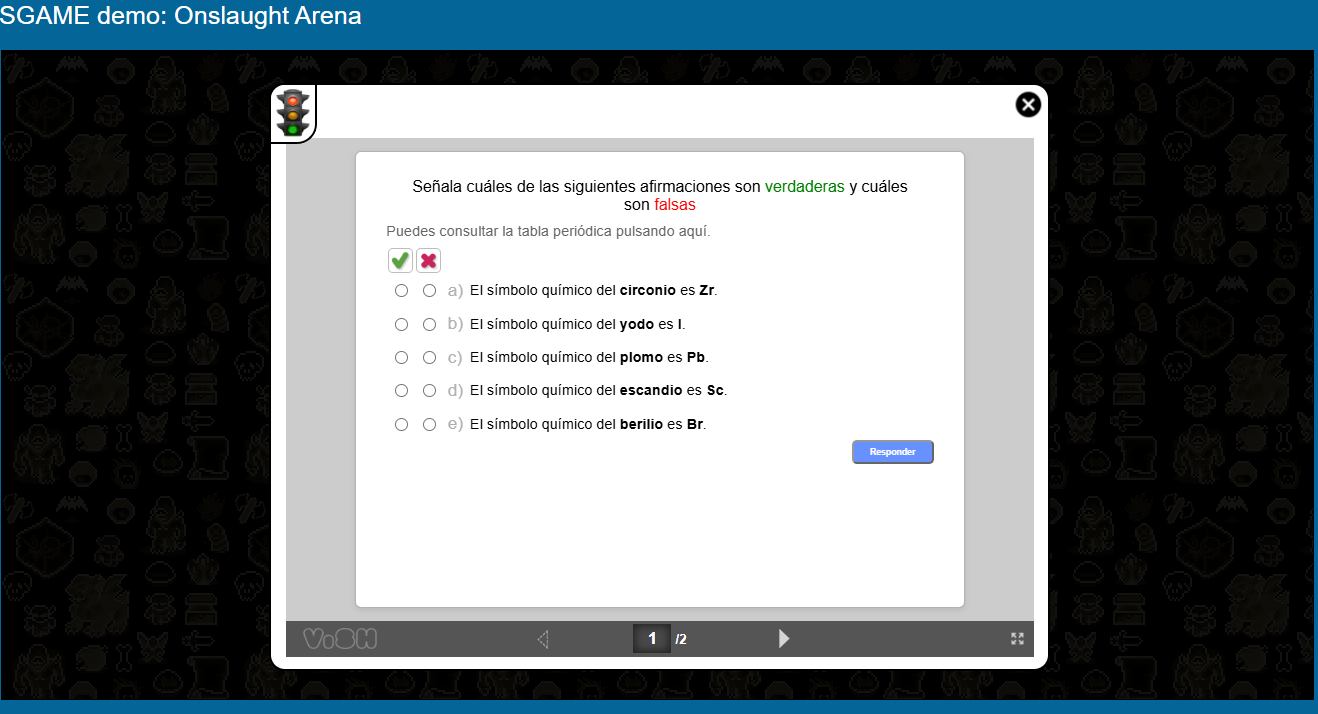
\includegraphics[width=0.8\textwidth]{figures/Related_Work/Sgame_gameplay.png}
    \caption{Educational game gameplay by Gordillo et al. (2020) \cite{sgame2020}}
    \label{fig:sgame2020_gameplay}
\end{figure}